\documentclass[12pt,a4paper]{article}
\usepackage[UTF8]{ctex}     %先引入ctex
\usepackage[utf8]{inputenc} %再引入inputenc
\usepackage{graphicx}
\usepackage{lazylatex}
\usepackage{amsmath}
\usepackage{bookmark}
\usepackage{enumerate}
\tcbuselibrary{documentation}
\graphicspath{{img/}}
% 边距
\geometry{left=2.0cm,right=2.0cm,top=2.0cm,bottom=3.0cm}
% 大题
\newenvironment{problems}{\begin{list}{}{\renewcommand{\makelabel}[1]{\textbf{##1}\hfil}}}{\end{list}}
% 小题
\newenvironment{steps}{\begin{list}{}{\renewcommand{\makelabel}[1]{##1.\hfil}}}{\end{list}}
% 答
\providecommand{\ans}{\textbf{答}:~}
% 解
\providecommand{\sol}{\textbf{解}.~}

\begin{document}
\title{\normalsize \underline{操作系统(D)}\\\LARGE第 3 次作业}
\author{李子龙 518070910095}
\date{\today}
\maketitle

\begin{problems}
    \item[3.1] Using the program shown in Figure 3.30, explain what the output will
    be at \texttt{LINE A}.
    \begin{code}{cpp}
#include <sys/types.h>
#include <stdio.h>
#include <unistd.h>
int value = 5;
int main()
{
    pid_t pid;
    pid = fork();
    if (pid == 0) { /* child process */
        value += 15;
        return 0;
    }
    else if (pid > 0) { /* parent process */
        wait(NULL);
        printf("PARENT: value = %d",value); /* LINE A */
        return 0;
    }
}
    \end{code}

    \ans \textbf{将会输出 \texttt{PARENT: value = 5}。}如果在第 10 行后添加:
\begin{code}{cpp}
    printf("CHILD: value = %d", value);
\end{code}
    那么将会补充输出:\texttt{CHILD: value = 20}。使用了 \texttt{fork()} 函数后,新进程复制了原来进程的地址空间,子进程修改了本进程内的 \texttt{value} 值,这种复制是真复制而不是引用复制,因此并不会改变父进程的 \texttt{value} 值,故原进程的 \texttt{value} 仍然是 5 。
    \item[3.2] Including the initial parent process, how many processes are created by
    the program shown in Figure 3.31?
    \begin{code}{cpp}
#include <stdio.h>
#include <unistd.h>
int main()
{
    /* fork a child process */
    fork();
    /* fork another child process */
    fork();
    /* and fork another */
    fork();
    return 0;
}
    \end{code}

    \ans \textbf{总进程数是 8 。} \texttt{fork()} 函数之后父子进程都会继续进行下面的代码片段。那么经过第一个 \texttt{fork()} 之后,变为 2 个进程,然后变为 4 个进程,最后变为 8 个进程。
    \item[3.4] Some computer systems provide multiple register sets. Describe what
    happens when a context switch occurs if the new context is already loaded into one of the register sets. What happens if the new context
    is in memory rather than in a register set and all the register sets are in
    use?

    \ans 对于拥有多寄存器组的机器,如果新的上下文就在某一个寄存器中的话,就直接改变当前寄存器组的指针。如果所有的寄存器组都满了,系统需要像以前一样在寄存器与内存之间进行数据复制。
    \item[3.8] Describe the actions taken by a kernel to context-switch between processes.
    
    \ans 内核发出中断请求,然后系统保存当前运行在 CPU 上的进程的上下文,内核运行结束后,恢复原进程。
    \item[3.10] Explain the role of the \texttt{init} (or \texttt{systemd}) process on UNIX and Linux
    systems in regard to process termination.

    \ans \texttt{init} 进程定期调用 \texttt{wait()},以便收集任何孤儿进程的退出状态,然后将其作为 \texttt{init} 的子进程,释放孤儿进程标识符和进程表示条目。
\end{problems}

% HW04
% \begin{problems}
%     \item[4.1] Provide three programming examples in which multithreading provides
%     better performance than a single-threaded solution.

%     \ans \begin{enumerate}
%         \item Web 服务器可能有多个客户并发访问它,如果一个 Web 服务器作为单个线程的传统进程来进行,那么一次只能处理一个请求,将会导致客户端的等待时间过长。而如果作为多进程的程序,则可以同时处理多个客户端的请求,这样就可以大大缩短等待时间。
%         \item 计算矩阵乘法时,如果按照传统的方式进行逐行逐列扫描计算,将会耗费大量的时间。而多线程可以采用矩阵分块的方式进行计算,从而大大缩短计算时间。
%         \item 合并排序又是一个很好的多线程程序例子,它可以使得多个子序列的排序同时进行而不是单线程的逐步等待,这样可以大大缩短排序时间。
%     \end{enumerate}
%     \item[4.4] What are two differences between user-level threads and kernel-level
%     threads? Under what circumstances is one type better than the other?
    
%     \ans \textbf{用户线程}位于内核之上,它的管理无需内核支持;而\textbf{内核线程}由操作系统来直接支持与管理。

%     当只需要进行内核指令时,内核进程更好一些。需要与用户进行交互的时候,用户进程更好一些。
%     \item[4.10] Which of the following components of program state are shared across
%     threads in a multithreaded process?
%     \begin{enumerate}[a.]
%         \item Register values
%         \item Heap memory
%         \item Global variables
%         \item Stack memory
%     \end{enumerate}

%     \ans 全局变量(c.)。每个线程都有自己的寄存器与堆栈。
%     \item[4.17] Consider the following code segment:
%     \begin{code}{cpp}
% pid_t pid;
% pid = fork();
% if (pid == 0) { /* child process */
%     fork();
%     thread_create( . . .);
% }
% fork();
%     \end{code} 
%     \begin{steps}
%         \item[a] How many unique processes are created?
%         \item[b] How many unique threads are created?
%     \end{steps}
    
%     \ans 共有 6 个不同进程产生,8个不同的线程产生。

%     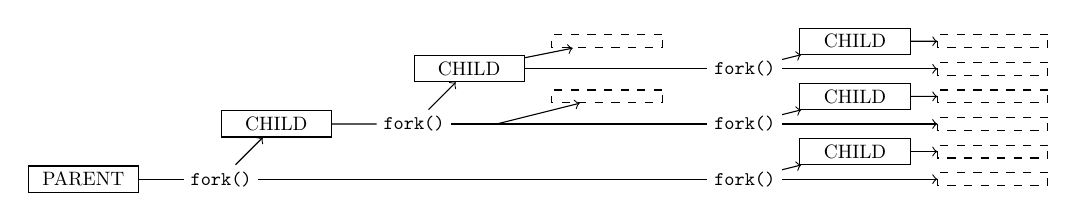
\begin{tikzpicture}[scale=0.7,every node/.style = {scale=0.7}]
\tikzstyle{process} = [minimum width=2cm,draw,];
\tikzstyle{thread} = [minimum width=2cm,draw,dashed]

\node [process] (v1) at (-1.5,0.5) {PARENT};
\node [process] (v2) at (2,1.5) {CHILD};
\node (v3) at (1,0.5) {\texttt{fork()}};

\draw  (v1) edge (v3);
\draw[->]  (v3) edge (v2);
\node (v4) at (4.5,1.5) {\texttt{fork()}};
\draw  (v2) edge (v4);
\node [process] (v5) at (5.5,2.5) {CHILD};
\draw[->]  (v4) edge (v5);
\node [thread] (v9) at (8,2) {};
\node [thread] (v7) at (8,3) {};
\draw[->]  (v5) edge (v7);
\draw[->] (6,1.5) -- (v9);
\node [process] (v11) at (12.5,1) {CHILD};
\node (v10) at (10.5,0.5) {\texttt{fork()}};
\draw  (v3) edge (v10);
\draw [->] (v10) edge (v11);
\node [thread] (v13) at (15,1) {};
\node [thread] (v12) at (15,0.5) {};
\draw[->]  (v10) edge (v12);
\draw[->]  (v11) edge (v13);
\node (v6) at (10.5,1.5) {\texttt{fork()}};
\draw  (v4) edge (v6);
\node (v8) at (10.5,2.5) {\texttt{fork()}};
\draw  (v5) edge (v8);
\node [process] (v15) at (12.5,2) {CHILD};
\node [process] (v14) at (12.5,3) {CHILD};
\draw[->]  (v8) edge (v14);
\draw[->]  (v6) edge (v15);
\node [thread] (v16) at (15,1.5) {};
\node [thread] (v17) at (15,2) {};
\node [thread] (v18) at (15,2.5) {};
\node [thread] (v19) at (15,3) {};
\draw [->]  (v6) edge (v16);
\draw [->]  (v15) edge (v17);
\draw [->] (v8) edge (v18);
\draw [->]  (v14) edge (v19);
\end{tikzpicture}


%     \item[4.19] The program shown in Figure 4.23 uses the Pthreads API. What would
%     be the output from the program at \texttt{LINE C} and \texttt{LINE P}?
%     \begin{code}{cpp}
% #include <pthread.h>
% #include <stdio.h>
% int value = 0;
% void *runner(void *param); /* the thread */
% int main(int argc, char *argv[])
% {
%     pid_t pid;
%     pthread_t tid;
%     pthread_attr_t attr;
%     pid = fork();
%     if (pid == 0) { /* child process */
%         pthread_attr_init(&attr);
%         pthread_create(&tid,&attr,runner,NULL);
%         pthread_join(tid,NULL);
%         printf("CHILD: value = %d",value); /* LINE C */
%     }
%     else if (pid > 0) { /* parent process */
%         wait(NULL);
%         printf("PARENT: value = %d",value); /* LINE P */
%     }
% }
% void *runner(void *param) {
%     value = 5;
%     pthread_exit(0);
% }
%     \end{code} 

%     \ans \texttt{CHILD: value = 5},\texttt{PARENT: value = 0}。因为线程会改变全局变量的值,而进程之间的变量是真复制,不是引用的,所以父进程的值仍然没有改变。
% \end{problems}

\end{document}
